%%  'printversion' pro sazbu verze pro tisk (nebarevné logo a odkazy,
%%  odkazy s uvedením adresy za odkazem, ne odkazy do rejstříku),
%%  jinak verze pro prohlížeč

%%  'biblatex' pro zapnutí podpory pro sazbu bibliografie pomocí
%%  BibLaTeXu, jinak je výchozí sazba v prostředí thebibliography

\documentclass[
  master,
  program=ainf,
  %  printversion,
  % biblatex,
  %  language=english,
  %  font=sans,
  % figures=false,
  tables=false,
  %  theorems,
  sourcecodes,
  glossaries,
  index
]{kidiplom}


\usepackage{float}

%% Název práce, česky a anglicky. Měl by se vysázet na jeden řádek.
\title{Srovnání JavaScriptových frameworků}
\title[english]{Comparison of JavaScript frameworks.}

%% Volitelný podnázev práce, česky a anglicky. Měl by se vysázet na
%% jeden řádek. Výchozí je prázdný.
\subtitle{}
\subtitle[english]{}

%% Jméno autora práce. Makro nemá nepovinný parametr pro uvedení
%% jazyka.
\author{Bc. David Hrůza}

%% Jméno vedoucího práce (včetně titulů). Makro nemá nepovinný
%% parametr pro uvedení jazyka.
\supervisor{RNDr. Martin Trnečka Ph.D.}

%% Volitelný rok odevzdání práce. Výchozí je aktuální (kalendářní)
%% rok. Makro nemá nepovinný parametr pro uvedení jazyka.
%\yearofsubmit{\the\year}

%% Anotace práce, včetně anglické (obvykle překlad z jazyka
%% práce). Jeden odstavec!
\annotation{Cílem této diplomové práce je srovnání reaktivních přístupů JavaScriptových frameworků
Vue, Svelte a SolidJS. Součástí je jednoduchá aplikace představující poštovního klienta v každém frameworku
pro demonstartivní účely.}

\annotation[english]{
  The goal of this thesis is to compare reactive data approach of JavaScript frameworks Vue, Svelte and SolidJS.
  Part of thesis is simple email client application written in each framework for demonstration purpose. 
}

%% Klíčová slova práce, včetně anglických. Oddělená (obvykle) středníkem.
\keywords{reaktivita; frontend; frameworky}
\keywords[english]{reactivity; frontend; frameworks}

%% Volitelná specifikace příloh textu práce, i anglicky. Výchozí je
%% 'elektronická data v systému katedry informatiky / electronic data
%% in system of department of computer science'.
%\supplements{nejlepší software všech dob}
%\supplements[english]{the best software of all times}

%% Volitelné poděkování. Stručné! Výchozí je prázdné. Makro nemá
%% nepovinný parametr pro uvedení jazyka.
\thanks{Mnohorát děkuji panu RNDr. Martinu Trnečkovi, Ph.D. za vedení a invostovaný čas. }

%% Cesta k souboru s bibliografií pro její sazbu pomocí BibLaTeXu
%% (zvolenou nepovinným parametrem biblatex makra
%% \documentclass). Použijte pouze při této sazbě, ne při (výchozí)
%% sazbě v prostředí thebibliography.
% \bibliography{bibliografie.bib}

%% Další dodatečné styly (balíky) potřebné pro sazbu vlastního textu
%% práce.
\usepackage{lipsum}
\usepackage{longtable}

\begin{document}
%% Sazba úvodních stran -- titulní, s bibliografickými údaji, s
%% anotací a klíčovými slovy, s poděkováním a prohlášením, s obsahem a
%% se seznamy obrázků, tabulek, vět a zdrojových kódů (pokud jejich
%% sazba není vypnutá).
\maketitle

%% Vlastní text závěrečné práce. Pro povinné závěry, před přílohami,
%% použijte prostředí kiconclusions. Povinná je i příloha s obsahem
%% elektronických dat.
%% -------------------------------------------------------------------

\section {Úvod}
S mírnou nadsázkou lze tvrdit, že není týden, kdy by se neobjevil nový frontendový
framework. Oblast frontendu je neustále velmi aktivně zlepšována. Jednou z hlavních
charakteristik frameworků je reaktivní systém frameworku. V této práci se podíváme 
na tři odlišené přístupy reaktivity. Reaktivitou se obecně myslí deklarativní přístup k 
programování. Pouhou změnou hodnoty proměnné se daná změna projeví všude, kde je 
proměnná použita.

\subsection{O autorovi}
V rychlosti si uvedeme autora, jelikož má předešlé zkušenosti v tomto oboru.
Autor diplomové práce pracuje pět let jako full--time full--stack developer.
Vyvíjí interní administrační portály a eshopové jádro. Po celou dobu kariéry
využívá na frontendu framework Vue \cite{vue}. V počátcích začínal na Vue 2 \cite{vue2} a v posledních
dvou letech Vue 3 \cite{vue}. Na backendu pracuje pouze v jazyce PHP \cite{php} s pomocí frameworku
Laravel \cite{laravel}. 

\subsection{O aplikaci Thessenger}
Zadání diplomové práce je demonstrovat přístupy několika frontendových
frameworků. Pro tento účel vznikla aplikace Thessenger. Jedná se aplikaci
simulující poštovního klienta.

Uživatelé se mohou registrovat do systému pomocí uživatelského jména a hesla.
Následně mohou ze systému odesílat v rámci systému ostatním uživatelům zprávy.
Zpráva může mít více příjemců. Místo konverzačních vláken se drží klasického
přístupu k emailu, kde každá zpráva udržuje historii konverzace v sobě.
Aplikace na pozadí hlídá existenci nových zpráv a upozorní na novou zprávu
červeným puntíkem v menu u položky \uv{Přijaté zprávy}.

\subsubsection{Mapa aplikace}
Stručný seznam stránek aplikace je následující:
\begin{itemize}
  \item Přihlášení
  \item Registrace
  \item Odeslání zprávy
  \item Přijaté zprávy
  \item Odeslané zprávy
  \item Detail zprávy
  \item Koš
\end{itemize}

\subsubsection{Registrace účtu}
Prvním krokem k získání přístupu do aplikace je registrace účtu. Jak můžeme vidět
na obrázku~\ref{fig:registration}, stačí vymyslet
uživatelské jméno a dostatečně silné heslo. Po vytvoření účtu je provedeno
automatické přihlášení a přesměrování do zabezpečené sekce aplikace.

\begin{figure}[H]
  \centering
  
\includegraphics[width=\textwidth]{graphics/thessenger_registration.png}
  \caption{Registrace účtu.}
  \label{fig:registration}
\end{figure}

\subsubsection{Nová zpráva}
Na obrázku~\ref{fig:new_message} vidíme stránku nová zpráva, na které můžeme vytvořit a odeslat zprávu.
Každá zpráva má svého odesílatele -- účet, ze které byla odeslána, několik
příjemců, předmět a obsah. 
Na obrázku~\ref{fig:new_message_multiselect} můžeme vidět možnost výběru
více příjemců. Seznam příjemců lze také filtrovat pro zúžení výběru, jak jde vidět na
obrázku~\ref{fig:new_message_filtration}.

\begin{figure}[H]
  \centering
  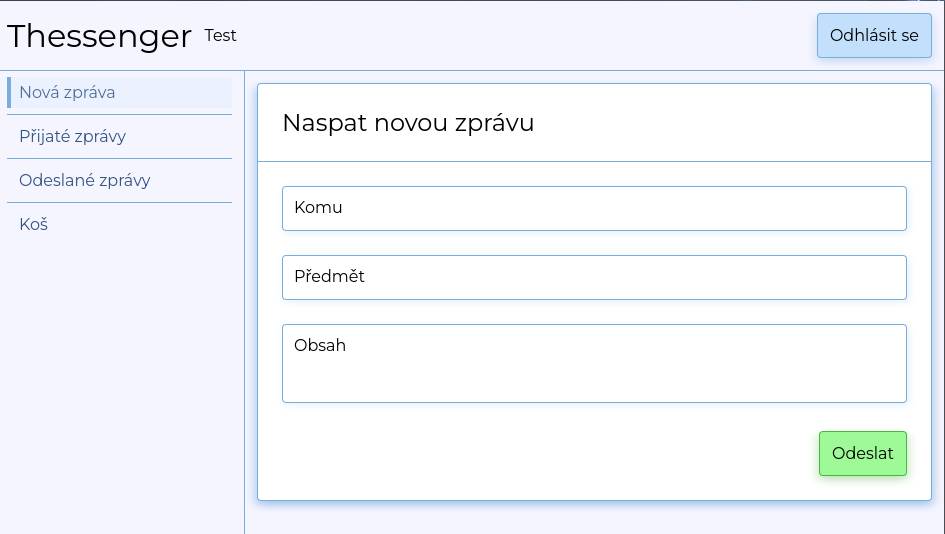
\includegraphics[width=\textwidth]{graphics/thessenger_new_message.png}
  \caption{Nová zpráva.}
  \label{fig:new_message}
\end{figure}

\begin{figure}[H]
  \centering
  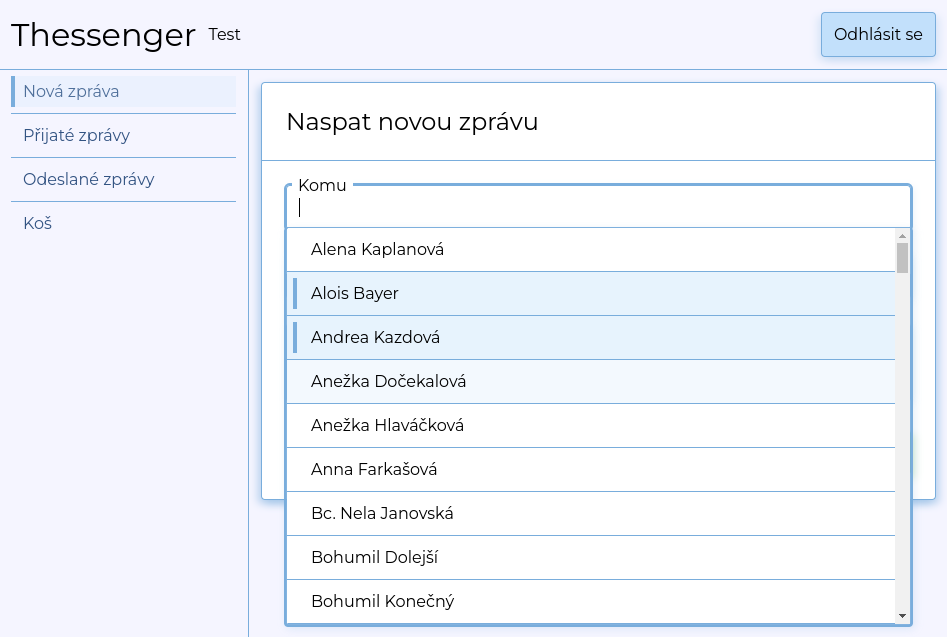
\includegraphics[width=\textwidth]{graphics/thessenger_new_message_multi_select.png}
  \caption{Nová zpráva výběr více příjemců.}
  \label{fig:new_message_multiselect}
\end{figure}

\begin{figure}[H]
  \centering
  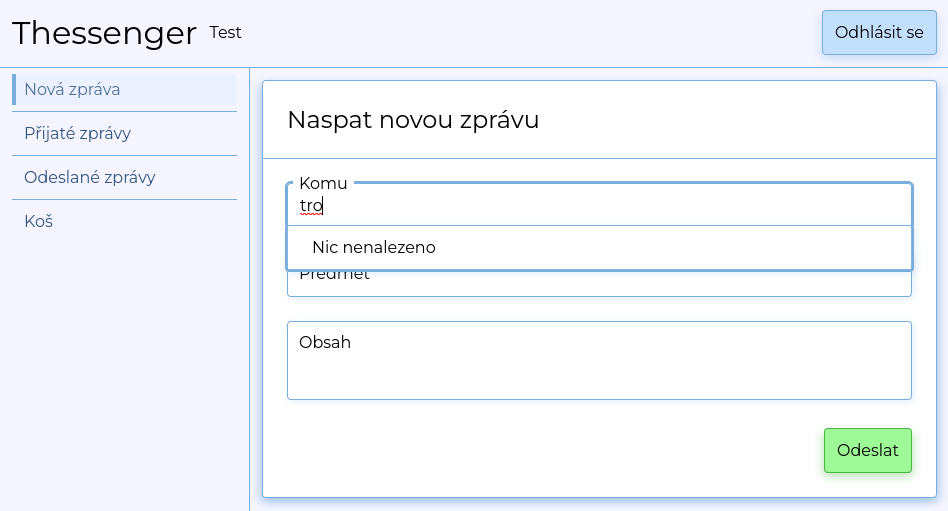
\includegraphics[width=\textwidth]{graphics/thessenger_new_message_nothing_found.png}
  \caption{Nová zpráva filtrace.}
  \label{fig:new_message_filtration}
\end{figure}

\subsubsection{Přijaté a odeslané zprávy}
Jedná se o totožné stránky s filtrovanými daty. Zobrazí se zde seznam všech
přijatých obrázek~\ref{fig:inobx} / odeslaných obrázek~\ref{fig:outbox} zpráv s možností přechodu na detail 
zprávy a možnosti smazání zprávy.

\begin{figure}[H]
  \centering
  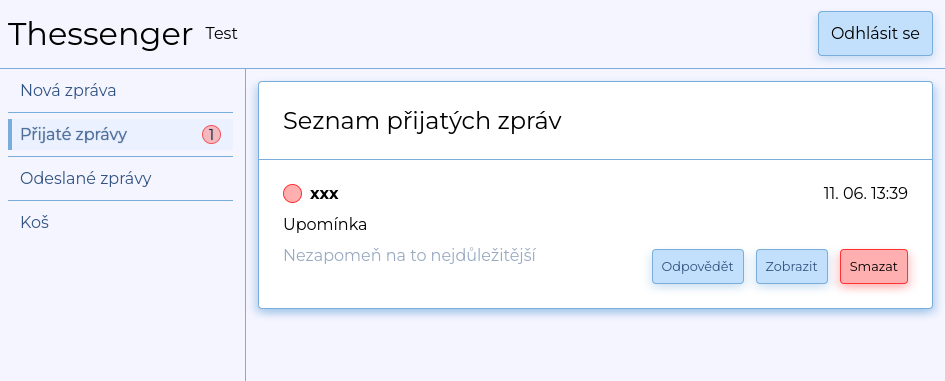
\includegraphics[width=\textwidth]{graphics/thessenger_inbox.png}
  \caption{Přijaté zprávy.}
  \label{fig:inobx}
\end{figure}

\begin{figure}[H]
  \centering
  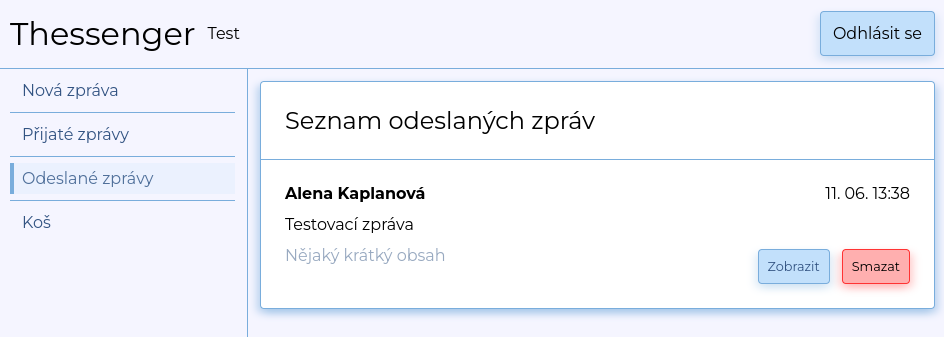
\includegraphics[width=\textwidth]{graphics/thessenger_outbox.png}
  \caption{Odeslané zprávy.}
  \label{fig:outbox}
\end{figure}

\subsubsection{Detail zprávy}
Detail zobrazí celý obsah zprávy, jak můžeme vidět na obrázku~\ref{fig:message_detail}. Obsah
zprávy může být triviálně formátován pomocí nových řádků a mezer. Samotný výpis je obalen v pre
značce a tudíž zachovává mezery.

\begin{figure}[H]
  \centering
  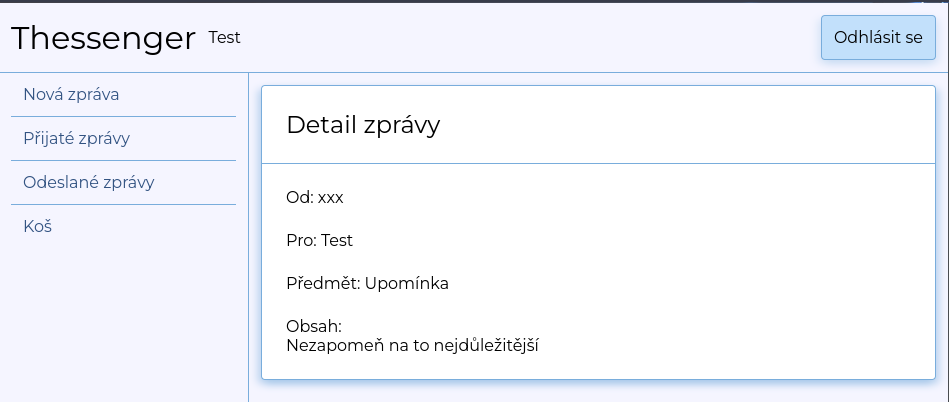
\includegraphics[width=\textwidth]{graphics/thessenger_message_detail.png}
  \caption{Detail zprávy.}
  \label{fig:message_detail}
\end{figure}

\subsubsection{Koš}
Stránka koše, zobrazená na obrázku~\ref{fig:bin}, nám umožňuje smazat položky navždy.

\begin{figure}[H]
  \centering
  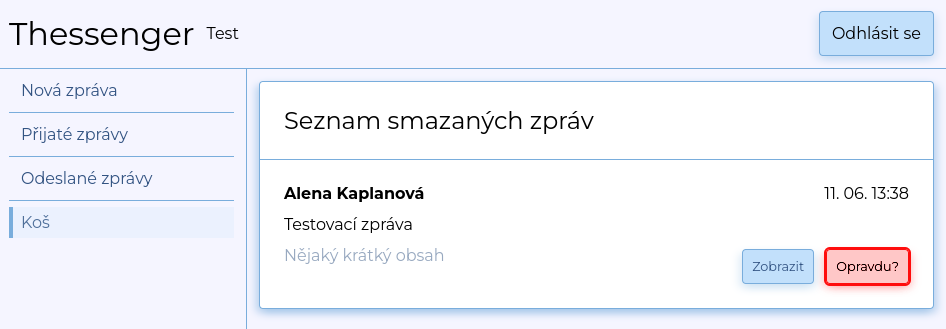
\includegraphics[width=\textwidth]{graphics/thessenger_bin.png}
  \caption{Koš.}
  \label{fig:bin}
\end{figure}

\newpage
\section{Implementace}
V rámci implementace byl dbán velký důraz na redukci redundantního kódu.
Vzhledem k tomu, že máme tři instance té samé aplikace psané pouze v různých
frameworcích je očekáváno velké množství stejného kódu.

\subsection{Adresářová struktura}
Aplikace je logicky rozdělena podle frameworků s dodatečnou složkou pro společný kód.
\begin{itemize}
  \item {\tt backend} - slouží pro manipulaci a ukládání dat
  \item {\tt common} - slučuje stejnou funkcionalitu frontendových frameworků
  \item {\tt solidjs} - implementace frontendu aplikace
  \item {\tt svelte} - implementace frontendu aplikace
  \item {\tt vue} - implementace frontendu aplikace
\end{itemize}

\subsection{Backend}
Na backend byl zvolen framework Laravel \cite{laravel}. Vývoj začal právě tímto projektem a k
ověření funkčnosti byly využity unit testy. Jediná zajímavá záležitost z
pohledu frontendu je vystavení všech dostupných endpointů do JSON API. Po
zavolání {\tt api/route/routes} dostaneme odpověď ve formátu zobrazeném ve zdrojovém kódu~\ref{code:routes}:

\begin{kicode}{JavaScript}{code:routes}{JSON seznam jednotlivých endpointů.}
{
  "auth.login":{
    "url": "api/auth/login",
    "method": "POST"
  }
}
\end{kicode}


Z těchto dat se pomocí skriptu vytvoří soubor {\tt routes.ts}, který obsahuje objekt ve formátu zobrazeném 
ve zdrojovém kódu~\ref{code:endpoints}.

\begin{kicode}{JavaScript}{code:endpoints}{Definice jednotlivých endpointů.}
  export const roues = {
    "message.send": {
      url: (message: string|number) => `/api/message/message/${message}/send`,
      method: "POST"
    }
  }
\end{kicode}

Díky tomu mají všechny frontendy staticky definované endpointy. Zároveň se z
jednotlivých URL pomocí regexu získá i informace o parametrech. Díky tomu 
se zmenšuje množství informací, které je nutné znát pro člověka na frontendu.
Pohledem na soubor s endpointy získá přehled o tom, co backend umožňuje a jaké
parametry jednotlivé endpointy požadují. Při změně endpointů by nám statická analýza
řekla, jestli využíváme všechny endpointy korektně. Navíc máme možnost na backendu
změnit v případě potřeby URL mez nutnosti úpravy frontendu.

\subsection{Common}
Adresář společných funkcionalit jednotlivých frontendových implementací. Dělí se
na tři větší celky.

\begin{itemize}
  \item {\tt css}
  \item {\tt ts/validation}
  \item {\tt ts/api}
\end{itemize}

Setkáváme se zde s nutností psaní framework-agnostického kódu. Nejprve
nastíníme problém, se kterým se musíme vypořádat. Každý framework řeší
reaktivní aktualizaci dat jinak.

\begin{kicode}{JavaScript}{code:reactive_variables}{Definice reaktivních proměnných.}
  // Vue příklad
  const count = ref(0);
  count.value = 42;

  // Svelte příklad
  let count = 0;
  count = 42;

  // SolidJS příklad
  const [count, setCount] = createSignal(0);
  setCount(42);
\end{kicode}

Jak je ze zdrojového kódu~\ref{code:reactive_variables} vidět, Vue \cite{vue} využívá funkci
{\tt ref} pro vytvoření reaktivního objektu,
SolidJS \cite{solidjs} používá funkci {\tt createSignal} pro získání getteru a setteru a Svelte \cite{svelte}
využívá reaktivitu na základě přiřazení. 

Zároveň má každý framework řešené komponenty\footnote{Komponenty slouží jako
  základní stavební blok. Definují, jak se mají vykreslit, mají svůj interní
  stav a dokáží upravit své chování na základě vstupních parametrů nebo
  oznámit změny pomocí událostí.} a komunikaci mezi nimi také jinak. Primárně
nás pro naše účely zajímá kontextuální předávání informací\footnote{V
  složitější struktuře komponent by mohlo být velmi náročné přeposílat data a
  události N úrovní hluboko. Kontextuální předávání dat pak umožňuje v
  komponentě poskytnout data a každá komponenta, která je jakkoli vzdáleným
  potomkem smí tato data získat.} mezi komponentami. Jednotlivé implementace 
  jsou demonstrovány ve zdrojovém kódu~\ref{code:contextual_api}.

  \begin{kicode}{JavaScript}{code:contextual_api}{Kontextuální API.}
  // Vue příklad v nadřazené komponentě
  provide('key', 42)
  // Vue příklad v podřazené komponentě
  const count = inject('key')

  // Svelte příklad v nadřazené komponentě
  setContext('key', 42)
  // Svelte příklad v podřazené komponentě
  const count = getContext('key')

  // SolidJS příklad v nadřazené komponentě
  export const useCount = useContext(createContext(42))
  // SolidJS příklad v podřazené komponentě
  const count = useCount()
\end{kicode}

Řešení samotného problému pak spočívá pouze ve využití getterů a setterů v
případě reaktivních dat. Pro potřeby kontextuálního api poskytneme pouze klíč a
funkce, které mají být sdíleny s potomky komponenty.

\subsubsection{CSS}
Všechny projekty by měly vypadat totožně. Dává tedy smysl mít pouze jednu
sdílenou sadu CSS pravidel. Je zajištěno, aby byla aplikace použitelná jak na
mobilních zařízeních, tak na desktopu.

\subsubsection{Ts/validation}
Definujeme systém pro validování formulářů. Primárně je tato funkcionalita
využita během registrace. Každý formulář poskytne svým potomků možnost
registrovat se jako vstupní políčko. Při odeslání formuláře jsou všechna pole
zkontrolována, zda je jejich validace platná. Pokud není, formulář nebude
odeslán.

\newpage
\section{Porovnávané frameworky}
Nejprve si představíme jednotlivé frameworky. Všechny mají společné jedno --
snaží se sblížit datovou a vizuální stránku. Pokud bychom tvořili větší
interaktivní stránku, velmi rychle dojdeme k závěru, že je vcelku náročné
sledovat kde se která data zobrazují a jakým způsobem se modifikují. Představme
si jednoduchý příklad, kdy chceme po stisknutí tlačítka navýšit hodnotu
interního čítače, který začíná na nule a zobrazit tuto hodnotu v divu. V čistém
JavaScriptu \cite{js} bychom museli po načtení stránky získat podle statických id
referenci na tlačítko a zobrazovací {\tt div}. Vytvořili bychom proměnnou {\tt count} a
nastavili ji na nulu. Museli bychom zaregistrovat odposlech události stisku
tlačítka myši na elementu tlačítka. V této události bychom mohli zároveň
upravit hodnotu zobrazovacího divu na současnou hodnotu proměnné {\tt count}. Už v
takto jednoduchém případě vidíme, že tento přístup není nejpřímočařejší.
Při pohledu na html nevidíme nic, co by nám říkalo, že tlačítko má navázanou
událost stisknutí tlačítka, nebo že obsah zobrazovacího divu bude upraven.
Naopak při pohledu na JavaScript \cite{js} zase nevidíme, s jakými prvky manipulujeme.

Zde přichází na pomoc frameworky. Každý definuje způsob, jak deklarativně
pracovat s daty přímo v šabloně. Základním stavebním blokem jsou komponenty.
Komponentu si můžeme představit jako třídu. Každá komponenta má svůj interní
stav a funkci, kterou se vykreslí. Když pak používáme komponenty je to jako
vytvoření instance třídy. Komponenty mají většinou životní cyklus. Tedy funkce,
které se volají při vytvoření nové instance (konstruktor) při vyjmutí z DOMu
(destruktor) a při aktualizaci DOMu (update).

Samotné komponenty nám umožňují vytvářet znovupoužitelné části kódu, ale
abychom opravdu vyřešili problém s neviditelným tokem dat, potřebujeme ještě
reaktivní data. Reaktivita je způsob, jak při změně proměnné implicitně
aktualizovat všechna místa, kde je tato proměnná použita. Nejedná se pouze o
šablony, ale například i proměnné odvozené. 

Dejme tomu, že máme reaktivní proměnnou {\tt x}. Můžeme vytvořit proměnnou {\tt y}, která
představuje například dvojnásobek proměnné {\tt x}. Pokud změníme hodnotu proměnné {\tt x},
musí se přepočítat i {\tt y} a všechna místa, kde je proměnná {\tt y} použita. Způsob, jakým
jednotlivé frameworky tento problém řeší se u každého zvoleného frameworku liší.

\subsection{Vue 3}
Vue \cite{vue} využívá k dosažení rekativity virtuální DOM a proxy objekty \cite{proxy}. K jednotlivým
pojmům se dostaneme po ukázce jednoduchého příkladu Vue komponenty.

\subsubsection{Komponenty}
Vue \cite{vue} má dva způsoby, jak definovat komponenty. Pomocí funkce a pomocí souboru 
s koncovkou {\tt .vue}. V případě souboru se jedná o takzvanou SFC.\footnote{Z anglického Single File Component}
Preferovaným způsobem dle dokumentace je psaní SFC komponent. Každá komponenta se skládá ze tří částí
zobrazených ve zdrojovém kódu~\ref{code:vue_sfc_overview}. První je šablona,
následuje kód a v poslední můžeme definovat styly.

\begin{kicode}{JavaScript}{code:vue_sfc_overview}{Vue SFC rozložení.}
  <template>Šablona</template>
  <script>Kód</script>
  <style>Styl</style>
\end{kicode}

V rámci kódu komponenty existují dvě API, jakými můžeme definovat reaktivní
data. V době Vue 2 \cite{vue2} existovalo pouze jediné -- takzvané Options API (zdrojový kód~\ref{code:vue_options_api}). V části kódu
byl zadefinovaný objekt, na kterém mohly existovat vlastnosti {\tt data}, {\tt computed},
{\tt methods} a jiné. Vlastnost {\tt data} definovala funkci, která byla zodpovědná ze
vytvoření počátečního stavu komponenty. Všechny vlastnosti vrácené v objektu
této funkce byly automaticky reaktivní a dostupné v šabloně. {\tt Data} byla dostupná
z metod přes klíčové slovo {\tt this}.

Options API je zastaralé. Reaktivní data nemohla být definována mimo komponentu
a logické celky\footnote{Data a metody pracující se těmito daty} byly 
fragmentovány na více místech. 

  \begin{kicode}{JavaScript}{code:vue_options_api}{Vue Options SFC rozložení.}
    <template>
      <span>{{a}}</span>
      <button @click="print">Print!</button>
    </template>
  
    <script>
      return default {
        data: () => ({
          a: ""
        }),
  
        methods: {
          print: () => {
            console.log(this.a);
          }
        }
      }
    </script>
  \end{kicode}

S příchodem Vue 3 \cite{vue} přišlo Composition API (zdrojový kód~\ref{code:vue_composition_api}). 
Definice reaktivních dat byla přesunuta do funkcí. Tento samotný krok přináší několik výhod. Můžeme 
definovat reaktivní data i mimo komponentu a nemusíme mít fragmentovanou strukturu SFC. Vše, co je
zadefinované v části kódu, je dostupné v šabloně. 


  \begin{kicode}{JavaScript}{code:vue_composition_api}{Vue Composition SFC rozložení.}
    <template>
      <span>{{a}}</span>
      <button @click="print">Print!</button>
    </template>
  
    <script setup>
      const a = ref("");
  
      const print = () => {
        console.log(a.value);
      }
    </script>
  \end{kicode}
  
Pro nás je nejzajímavější funkce {\tt ref}, která definuje reaktivní proměnnou.
Vytvoří to pro nás zástupce, na kterém je vlastnost {\tt value}, přes kterou můžeme
získat obsah proměnné nebo jej změnit. V šabloně není nutné volat {\tt .value} na
reaktivních proměnných - je to zajištěno automaticky.

Aby mohlo Vue \cite{vue} hlídat změny reaktivních dat, vrací funkce {\tt ref} Proxy objekt \cite{proxy}. Proxy
objekty \cite{proxy} jsou hojně využívány pro sledování změn reaktivních proměnných i mimo framework
Vue \cite{vue}, proto si je v rychlosti představíme.

\subsubsection{Proxy}

V jednoduchosti má každý objekt v jazyce JavaScript \cite{js} základní množinu metod \cite{default_methods}. Část této množiny můžeme vidět
ve zdrojovém kódu ~\ref{code:default_methods}.
Mezi ně patří metody {\tt get} a {\tt set}, které jsou volány při čtení a zápisu vlastností.

\begin{kicode}{JavaScript}{code:default_methods}{Základní metody objektů.}
  const test = {a: 42};
  console.log(test.a); // Na pozadí spustí metodu get
  test.a = 21; // Na pozadí spustí metodu set
\end{kicode}

Proxy nám umožní vytvořit zástupce objektu. Zástupce je nový objekt, u kterého
můžeme přetížit chování všech základních metod objektu. Tedy kromě pozorování 
změn můžeme i změnit nastavovaná data. Proxy je primitivum jazyka JavaScript \cite{js}, tedy
pro vytvoření nové proxy nám satčí zavolat {\tt new Proxy}, jak můžeme vidět ve zdrojovém kódu~\ref{code:new_proxy}

\begin{kicode}{JavaScript}{code:new_proxy}{Vytvoření proxy.}
  const target = {};

  const proxy = new Proxy(target, options);
\end{kicode}

Druhým parametrem konstruktoru Proxy je objekt definující přetížení základních metod \cite{default_methods}. 
Definici takového objektu můžeme vidět ve zdrojovém kódu~\ref{code:proxy_methods}.

\begin{kicode}{JavaScript}{code:proxy_methods}{Přetížení metod pomocí Proxy.}
  const options = {
    get(target, prop, receiver) {
      return Reflect.get(...arguments);
    },

    set(obj, prop, newval) {
      Reflect.set(...arguments)
    }
  };
\end{kicode}

V případě, že chceme zachovat výchozí chování přetížené metody, máme k dispozici objekt
{\tt Reflect}, který definuje některé z metod, které umožňují Proxy přetížit.


\subsubsection{Proxy ve Vue}

Se znalostí chování Proxy definujeme naivní implementaci funkce {\tt ref} ve zdrojovém kódu~\ref{code:vue_ref_definition}. 

\begin{kicode}{JavaScript}{code:vue_ref_definition}{Naivní implementace funkce ref.}
  const ref = (value) => {
    return new Proxy({ value: value }, {
      set(obj, prop, newval) {
        rebuildComponent();
        return Reflect.set(...arguments);
      }
    })
  }
\end{kicode}

Při zavolání naší funkce {\tt ref} dostáváme objekt, na kterém je definovaná vlastnost {\tt value}. 
Každá změna této vlastnosti zavolá funkci {\tt rebuildComponent}, která je zodpovědná za
opravení všech míst, kde se s proměnnou pracuje. V případě Vue \cite{vue} tato funkce způsobí
kontrolu virtuálního DOMu oproti reálnému DOMu a sestaví se sada opravných změn, které
opraví reálný DOM tak, ať odpovídá virtuálnímu.

\subsubsection{Options API}

Mimo funkci {\tt ref} máme k dispozici ještě {\tt computed} a {\tt reactive}. Funkce {\tt computed} bere jako parametr
funkci, která musí vrátit hodnotu. Kdykoli je použita v rámci této funkce reaktivní proměnná, 
dojde znovu ke spuštění funkce vždy, když se některá z reaktivních proměnných změní.
Použití můžeme vidět ve zdrojovém kódu~\ref{code:vue_computed}.

\begin{kicode}{JavaScript}{code:vue_computed}{Použití computed funkce.}
  const x = ref(2);
  const xPow2 = computed(() => x.value * x.value)
\end{kicode}

V případě, kdy potřebujeme vytvořit několik reaktivních proměnných najednou, můžeme pomocí
funkce {\tt reactive} zreaktivnit všechny vlastnosti na objektu, jak můžeme vidět ve zdrojovém kódu~\ref{code:vue_use_of_reactive}.

\begin{kicode}{JavaScript}{code:vue_use_of_reactive}{Použití reactive funkce.}
  const data = reactive({
    x: 42,
    y: 41
  })

  data.y = 42;
\end{kicode}

U reaktivních objektů nepotřebujeme volat {\tt .value}. Samotná modifikace i jakkoli hlubokých
objektů je automaticky detekována. 

Nyný máme k dispozici reaktivní data, odvozené proměnné, ale občas potřebujeme reagovat
na změnu reaktivní proměnné nějakým vedlejším efektem. Například vždy, když se změní
proměnná, vypsat její hodnotu do konzole. K tomu nám slouží funkce {\tt watch}. Ta bere jako 
první argument reaktivní proměnnou a druhý argument funkci, která se spustí vždy při změně
prvního argumentu. Použití můžeme vidět ve zdrojovém kódu~\ref{code:vue_watch}.

\begin{kicode}{JavaScript}{code:vue_watch}{Hlídání změn.}
  const x = ref(0);
  watch(x, (value) => console.log(value));
  x.value = 42;
\end{kicode}

\subsection{Svelte}
Svelte \cite{svelte} přistupuje k celému problému reaktivity jinak. Místo virtuálního DOMu přidává kompilační
krok. Místo Proxy \cite{proxy} hlídá změny na základě přiřazení.

\subsubsection{Komponenty}

Svelte \cite{svelte} definuje komponenty podobným způsobem jako jsou Vue SFC. Každá komponenta se skládá,
stejně jako Vue \cite{vue}, ze tří částí definovaných ve zdrojovém kódu~\ref{code:svelte_sfc} -- kód, šablona a styl.
S tím rozdílem, že šablona není obalená v template značce.

\begin{absolutelynopagebreak}
\begin{kicode}{JavaScript}{code:svelte_sfc}{Svelte SFC rozložení.}
  <script>Kód</script>
  <div>Šablona</div>
  <style></style>
\end{kicode}
\end{absolutelynopagebreak}

\subsubsection{Reaktivita}

Na první pohled vypadá kód Svelte komponent ve zdrojovém kódu~\ref{code:svelte_simple_code} jako klasický JavaScript \cite{js}. Deklarujeme proměnnou {\tt count},
klasicky ji můžeme upravit a následně ji použít v šabloně.

\begin{kicode}{JavaScript}{code:svelte_simple_code}{Svelte příklad.}
  <script>
    let count = 0;

    function handleClick() {
      count += 1;
    }
  </script>

  <button on:click={handleClick}>
    Clicked {count} {count === 1 ? 'time' : 'times'}
  </button>
\end{kicode}

Až téměř magicky bude vše fungovat přesně dle očekávání. Stejně jako Vue \cite{vue} umožňuje Svelte \cite{svelte} definovat
odvozené proměnné, které můžeme vidět ve zdrojovém kódu~\ref{code:svelte_computed}. Zápis je poněkud nezvyklý, ale umožňuje nám definovat jak odvozené proměnné, tak
hlídat změny stavu stejnou syntaxí. 

  \begin{kicode}{JavaScript}{code:svelte_computed}{Svelte odvozené proměnné.}
    <script>
      let count = 0;
      $: doubled = count * 2;

      $: {
        console.log('the count is ' + count);
      }
    </script>
  \end{kicode}

Kdykoli se proměnná {\tt count} změní, nejen že se přepočítá proměnná {\tt doubled}, ale zároveň se do konzole
vypíše text.

Avšak ne všechno jde takto hladce. Musíme si dávat pozor na to, abychom vždy provedli přiřazení.
Nejvíce na toto trpí pole, kde přidání nového záznamu musí být následováno přiřazením pole
samo do sebe, nebo s pomocí ES6\footnote{Z anglického ECMAScript 6, což je specifikace definující standard jazyka JavaScript}. Oba přístupy jsou demonstrovány ve zdrojovém kódu~\ref{code:svelte_problematic_array}.

  \begin{kicode}{JavaScript}{code:svelte_problematic_array}{Svelte problémové části.}
    <script>
      let numbers = [];

      function addNumber() {
        numbers.push(numbers.length + 1);
        numbers = numbers;
      }
      // nebo
      function addNumber() {
        numbers = [...numbers, numbers.length + 1];
      }
    </script>
  \end{kicode}


U objektů si taktéž musíme dávat pozor na to, aby se vždy vyskytl aktualizovaný objekt na levé části přiřazení.
Jinými slovy následující zdrojový kód~\ref{code:svelte_object_ok} je v pořádku.

  \begin{kicode}{JavaScript}{code:svelte_object_ok}{Svelte přiřazení objektů správně.}
    <script>
      const x = { y: { z: 42 }};
      x.y.z = 21;
    </script>
  \end{kicode}

Ale v tomto zdrojovém kódu~\ref{code:svelte_object_nok} by změna detekována nebyla.

  \begin{kicode}{JavaScript}{code:svelte_object_nok}{Svelte přiřazení objektů špatně.}
    <script>
      const x = { y: { z: 42 }};
      const temp = x.y;
      temp.z = 21;
      // nebo
      function test(thing) {
        thing.y.z = 21;
      }
      test(x);
    </script>
  \end{kicode}


\subsubsection{Reaktivita mimo komponenty}

Aby toho nebylo málo, změny přiřazením jsou detekovány pouze v rámci Svelte komponent. Pokud bychom
chtěli mít reaktivní proměnnou mimo komponentu, má pro to Svelte \cite{svelte} připravené takzvané sklady.
\footnote{Z anglického názvu stores} 

Sklady jsou obyčejné objekty s metodou {\tt subscribe}, která umožní komukoli být upozorněn v případě změny
hodnoty skladu. Metoda {\tt subscribe} vrací funkci k zrušení sledování změn. Existují tři typy 
skladů -- pro zápis (writable), pro čtení (readable) a odvozené (derived).

Zapisovatelné sklady jsou obdobou deklarace reaktivní proměnné pomocí funkce {\tt ref} z Vue \cite{vue}. Kromě povinné metody
subscribe obsahují také metody {\tt set} a {\tt update} k modifikaci stavu. Jednoduché využití skladu můžeme vidět
ve zdrojovém kódu~\ref{code:svelte_stores}.

  \begin{kicode}{JavaScript}{code:svelte_stores}{Svelte zapisovatelný sklad.}
    // js soubor
    export const count = writable(0);
    export const addOne = () => count.update((value) => value + 1);
    // svelte komponenta
    <script>
      let countValue;

      count.subscribe(value => {
        countValue = value;
      });
    </script>
    <div>{countValue}</div>
  \end{kicode}

Tento způsob zápisu je docela zdlouhavý a zároveň náchylný k chybě. V ukázkovém příkladu jsme totiž zapomněli
při zničení komponenty zavolat \\{\tt unsubscribe}. Mohlo by tedy dojít postupem času k úniku paměti. Svelte \cite{svelte} má pro
použití skladů syntaktický cukr. Místo manuálního zápisu a odpisu pro sledování změn můžeme v rámci komponenty
použít sklad s prefixem {\tt \$}, jak je demonstrováno ve zdrojovém kódu~\ref{code:svelte_store_with_sugar}.
Ukázkový příklad~\ref{code:svelte_stores} se tím zjednoduší a automaticky se zajistí volání metod {\tt subscribe} a {\tt unsubscribe}.

  \begin{kicode}{JavaScript}{code:svelte_store_with_sugar}{Svelte zapisovatelný sklad se syntaktickým cukrem.}
    // js soubor
    export const count = writable(0);
    export const addOne = () => count.update((value) => value + 1);
    // svelte komponenta
    <script>
    </script>
    <div>{$countValue}</div>
  \end{kicode}

Dále můžeme vytvářet sklady, které slouží pouze pro čtení. Tento typ skladů se může využít například pro
reaktivní čas nebo pozici myši. Funkce {\tt readable} bere dva parametry. Prvním je výchozí hodnota a druhým funkce,
která dostane jako parametr aktualizační funkci a vrací funkci pro zrušení skladu. Definici takového skladu
vidíme ve zdrojovém kódu~\ref{code:svelte_readable_store}, kde definujeme sklad pro reaktivní zobrazení aktuálního času.

\begin{absolutelynopagebreak}
  \begin{kicode}{JavaScript}{code:svelte_readable_store}{Svelte sklad pro čtení poskytující aktuální čas.}
    export const time = readable(new Date(), (set) => {
      const interval = setInterval(() => {
        set(new Date());
      }, 1000);

      return () => {
        clearInterval(interval);
      };
    });
  \end{kicode}
\end{absolutelynopagebreak}

Posledním typem je odvozený sklad. Funkce {\tt derived} opět bere dva parametry. Prvním je sklad, ze kterého
má být hodnota odvozená a druhý je funkce pro výpočet odvozené hodnoty.

\subsection{SolidJS}

Poslední framework je v určitém smyslu na pomezí mezi předchozími frameworky. Jako Vue \cite{vue} využívá Proxy objektů \cite{proxy}
k hlídání změn\footnote{Pro hlídání zanořených změn} a jako Svelte \cite{svelte} se vyhýbá virtual DOMu.

\subsubsection{Komponenty}

Komponenty jsou zde prosté funkce, které vrací JSX. Z tohoto pohledu je SolidJS \cite{solidjs} velmi podobný Reactu \cite{react}.
Nemáme tedy žádné speciální soubory s koncovkou {\tt .solid}. Místo toho máme soubory s koncovkou {\tt .tsx} pro
TypeScript \cite{ts} nebo {\tt .jsx} pro JavaScript \cite{js}. Každý takový soubor může obsahovat i několik komponent. Samotná
funkce definující komponentu slouží jako konstruktor. Je volaná pouze jednou. Komponentu pro zobrazení
čítače můžeme vidět ve zdrojovém kódu~\ref{code:solid_component}.

  \begin{kicode}{JavaScript}{code:solid_component}{SolidJS komponenta.}
    export const Counter = () => {
      const [count, setCount] = createSignal(0);

      const addOne = () => setCount((value) => value + 1);

      return <button onClick={addOne}> {count()} </button>;
    }
  \end{kicode}

\subsubsection{Reaktivita}

Máme k dispozici tři hlavní primitiva, které nám umožňují definovat reaktivní data. Obdobou funkce {\tt ref}
z Vue \cite{vue} je zde funkce {\tt createSignal}. Místo toho, aby nám vrátila objekt, vrací dvojici {\tt getter} a {\tt setter}.
Dále máme funkci {\tt createMemo}, které nám umožňuje definovat odvozenou proměnnou a {\tt createEffect}, kterou 
můžeme využít pro sledování změn a aplikování vedlejšího efektu. Použití základních funkcí můžeme vidět ve 
zdrojovém kódu~\ref{code:solid_reactivity}.

  \begin{kicode}{JavaScript}{code:solid_reactivity}{SolidJS reaktivita.}
    const [count, setCount] = createSignal(0);
    createEffect(() => console.log(count()));
    const doubleCount = createMemo(() => count() * 2);
  \end{kicode}

Dále si přiblížíme způsob, jakým SolidJS \cite{solidjs} hlídá změny. Jádrem celého systému je globální zásobník, který
se využívá pro automatické detekování závislostí. Ve výsledku to znamená, že není zapotřebí proxy objektů
k docílení reaktivity.

Samotná funkce {\tt createSignal} vytvoří lexikálně uzavřené prostředí, ve kterém existuje hodnota
signálu a seznam odběratelů změn. Vrací nám zmíněné dvě funkce pro čtení a zápis interní hodnoty.
Triviální implementace funkce {\tt createSignal} může být například definována, jako ve zdrojovém 
kódu~\ref{code:solid_signal}.

  \begin{kicode}{JavaScript}{code:solid_signal}{SolidJS createSignal.}
    function createSignal(value) {
      const subscribers = new Set();

      const read = () => {
        return value;
      };

      const write = (nextValue) => {
        value = nextValue;
      };

      return [read, write];
    }
  \end{kicode}

Nyní ke způsobu, jakým dochází k registrování odběratelů změn. Vždy, před spuštěním funkce poskytnuté do 
funkce \\{\tt createEffect} nebo {\tt createMemo} se zaregistrují jako odběratelé do globálního zásobníku. Každé spuštění
{\tt getteru} signálu následně způsobí zkontrolování, zda všichni ze zásobníku jsou registrování v interním seznamu
odběratelů daného signálu. Rozšířená verze tedy může být definována jako ve zdrojovém kódu~\ref{code:solid_signal_with_registration}.

\begin{absolutelynopagebreak}
  \begin{kicode}{JavaScript}{code:solid_signal_with_registration}{SolidJS createSignal s automatickou registrací odběratelů.}
    function createSignal(value) {
      const subscribers = new Set();

      const read = () => {
        const listener = getCurrentListener();
        if (listener) subscribers.add(listener);
        return value;
      };

      const write = (nextValue) => {
        value = nextValue;
        for (const sub of subscribers) sub.run();
      };

      return [read, write];
    }
\end{kicode}
\end{absolutelynopagebreak}

Tím máme zajištěné, že při každé změně signálu jsou obeznámeni všichni odběratelé a jejich hodnoty jsou
přepočítány.

Samotné šablony komponent se chovají velmi podobně. JSX je v rámci kompilace převedeno na renderovací
funkci, která je schopná detekovat, které části DOMu mají být upraveny při změně kterého signálu.
Jediná podmínka, která musí být splněna pro správné chování komponent je volání funkce {\tt createRoot}. 
Ta je zodpovědná za úklid po zaniklých komponentách aby nedocházelo k úniku paměti. Tato funkce se 
automaticky volá v rámci {\tt render} funkce, která je doporučeným způsobem, jak vytvořit vstupní bod
SolidJS \cite{solidjs} aplikace.

Na rozdíl od frameworků využívajících virtuální DOM, kde dochází k renderovacímu cyklu, při němž 
může dojít během jedné aktualizace k více změnám, SolidJS \cite{solidjs} využívá synchronní aktualizace. Tedy například
pokud bychom aktualizovali dvě proměnné {\tt name} a {\tt surname} ve zdrojovém kódu~\ref{code:solid_sync_reactivity},
ihned po aktualizaci {\tt name} bude již změna aplikována do DOMu.

\begin{absolutelynopagebreak}
  \begin{kicode}{JavaScript}{code:solid_sync_reactivity}{SolidJS synchronní reaktivní aktualizace.}
    export const Greeter = () => {
      const [name, setName] = createSignal("Honza");
      const [surname, setSurname] = createSignal("Novák");

      const fullName = () => {
        const result = `${name()} ${surname()}`;
        console.log(`Full name is: ${result}`);
        return result;
      }

      const update = () => {
        setName("Pepa");
        setSurname("Dvořák");
      }
      
      return <button onClick={update}>{fullName()}</button>
    }
\end{kicode}
\end{absolutelynopagebreak}

To může mít za následek vícenásobné vyhodnocení odvozených funkcí. Z uvedeného zdrojového kódu~\ref{code:solid_sync_reactivity} bychom po
stisknutí tlačítka viděli v konzoli dva záznamy. Prvním by byl \uv{Pepa Novák} a druhý \uv{Pepa Dvořák}.
Abychom se této situaci vyvarovali, můžeme využít funkci {\tt batch}, která odloží aktualizace po skončení
všech modifikací. Viz zdrojový kód~\ref{code:solid_batch}.

  \begin{kicode}{JavaScript}{code:solid_batch}{SolidJS synchronní reaktivní aktualizace s batchingem.}
    export const Greeter = () => {
      ...
      const update = () => batch(() => {
        setName("Pepa");
        setSurname("Dvořák");
        })
        ...
        }
      \end{kicode}

Pokud bychom opomenuli odvozené funkce, problém okamžitého projevení do DOMu zmizí. Naopak se občas
dostáváme do situace například ve Vue \cite{vue}, kdy si musíme počkat na aktualizaci DOMu například abychom mohli
správně určit šířku nebo výšku elementu. Díky tomu, že SolidJS \cite{solidjs} nemusí porovnávat virtuální DOM s reálným,
si může dovolit provést změnu okamžitě, protože cena této operace je stejná, ať se jedná o samostatnou změnu
nebo o sadu změn. 
    
\subsubsection{Proxy objekty}
Na začátku jsme se řekli, že je SolidJS \cite{solidjs} podobný Vue \cite{vue} právě v tom, že využívá Proxy objekty. Pokud ale
signály nevyužívají Proxy objekty \cite{proxy} a signály jsou základním stavebním blokem reaktivního systému jako
funkce {\tt ref} z Vue \cite{vue}, k čemu jsou zapotřebí?

Pravdou je, že nejsou striktně potřebné. Jsme schopni psát celý systém bez Proxy objektů \cite{proxy}.
Někdy nám mohou ale ušetřit práci. Představme si aplikaci, která eviduje nákupní seznam. Můžeme přidat
záznam a následně jej v seznamu označit za hotový. Existují z pohledu reaktivity tři způsoby, jak takovou 
aplikaci implementovat.

Prvním je naivní implementace zobrazena ve zdrojovém kódu~\ref{code:solid_naive_array}. Vytvoříme signál {\tt list}
reprezentující seznam. Přidání záznamu spočívá ve 
vytvoření nového pole, kde na konec přidáme nový záznam. Dosud je vše v pořádku. SolidJS \cite{solidjs} se postará o to,
aby byl DOM modifikován minimalisticky, tedy pouze přidá nový element na konec. Dále po kliknutí na záznam
chceme tento záznam označit za vyřešený. Můžeme stávající seznam projít, a element, na který jsme klikli,
nahradit novým elementem, který bude mít nastavený příznak, že byl vyřešen. Pro SolidJS \cite{solidjs} to je ale vytvoření
nového elementu a zrušení původního. Místo označení textu například pomocí css bude v DOMu nahrazen celý
element. Toto není nejefektivnější, jelikož je celá komponenta zahozena a znovu vytvořena kvůli minimální
změně.

  \begin{kicode}{JavaScript}{code:solid_naive_array}{SolidJS naivní modifikace pole.}
    export const App = () => {
      const [getList, setList] = createSignal([])
      ...
      const addItem = (text) => {
        setList([...getList(), { id: ++itemId, text, completed: false }]);
      }
      const toggleItem = (id) => {
        setList(getList().map((item) => (
          item.id !== id ? item : { ...item, completed: !item.completed }
        )));
      }

      return (
        <>
          ...
          <For each={getList()}>
            {(item) => {<span>{item.text} {item.completed ? ' - Hotovo' : ''</span>} }}
          </For>
        </>
      );
    };
\end{kicode}

Druhým způsobem, zobrazeným ve zdrojovém kódu~\ref{code:solid_signal_array}, jak se s touto situací vypořádat 
je využití signálu na úrovni záznamu. Každé vytvoření
záznamu vytvoří signál {\tt completed}. Místo samotné hodnoty pošleme do objektu {\tt getter} a {\tt setter} této hodnoty.
Při přepnutí stavu záznamu můžeme zavolat poskytnutý {\tt setter}, tím dojde pouze k úpravě potřebné pro projevení
změny stavu. Celá komponenta nebude zničena a znovu vytvořena. Toto řešení je lepší, ale musíme kvůli němu
upravit také komponentu pro výpis záznamů. Místo toho abychom pouze vypsali hodnotu {\tt completed} musíme volat
{\tt getter}.

  \begin{kicode}{JavaScript}{code:solid_signal_array}{SolidJS modifikace pole s pomocí signálu.}
    export const App = () => {
      const [getList, setList] = createSignal([])
      ...
      const addItem = (text) => {
        const [completed, setCompleted] = createSignal(false); 
        setList([...getList(), { id: ++itemId, text, completed, setCompleted }]);
      }
      const toggleItem = (id) => {
        const item = getList().find((item) => item.id === id);
        if (item) item.setCompleted(value => !value)
      }

      return (
        <>
          ...
          <For each={getList()}>
            {(item) => {<span>{item.text} {item.completed() ? ' - Hotovo' : ''</span>} }}
          </For>
        </>
      );
    };
\end{kicode}

Posledním způsobem, zobrazeným ve zdrojovém kódu ~\ref{code:solid_store_array}, je využití skladu. 
I SolidJS \cite{solidjs} má své sklady, pouze z jiného důvodu, než Svelte \cite{svelte}. Ve Svelte \cite{svelte}
jsme je využívali ke zprovoznění reaktivity mimo komponenty. Zde takový problém nemáme. Funkci {\tt createSignal}
můžeme volat odkudkoli. Sklady nám v rámci SolidJS \cite{solidjs} pomohou s hloubkovou reaktivitou. V předchozím řešení 
jsme museli upravit komponentu pro zobrazení záznamů, jelikož jsme místo obyčejné hodnoty dostali {\tt getter}.
Pokud místo signálu pro reprezentaci seznamu využijeme skladu, můžeme pracovat se záznamem jako v naivní
implementaci. SolidJS \cite{solidjs} se postará o vytvoření potřebných signálů na pozadí. Vyváření signálu se navíc provádí
pouze pro vlastnosti záznamu, které jsou sledovány, líně až v okamžiku potřeby. Tímto máme řešení, které
je definováno podobně přímočaře jako naivní řešení, ale je stejně efektivní jako druhé řešení.

\begin{absolutelynopagebreak}
  \begin{kicode}{JavaScript}{code:solid_store_array}{SolidJS modifikace pole s pomocí skladu.}
    export const App = () => {
      const [list, setList] = createStore([])
      ...
      const addItem = (text) => {
        setList([...list, { id: ++listId, text, completed: false }]);
      }
      const toggleItem = (id) => {
        setList(list => list.id === id, "completed", completed => !completed);
      }

      return (
        <>
          ...
          <For each={getList()}>
            {(item) => {<span>{item.text} {item.completed ? ' - Hotovo' : ''</span>} }}
          </For>
        </>
      );
    };
\end{kicode}
\end{absolutelynopagebreak}

Tedy programátor může rozhodnout, zda chce využít Proxy objektů k zjednodušení definice komponent, nebo zda
se chce využití Proxy objektů vyhnout. Starší prohlížeče Proxy objekty nemusejí podporovat, proto se SolidJS \cite{solidjs}
hodí i pro vývoj aplikací do různých embed řešení, které mají zastaralý software.

\newpage
\section{Srovnání frameworků}
V této kapitole srovnáme jednotlivé frameworky mezi sebou. Nejprve se na ně podíváme z pohledu programátora.
Následně se podíváme na vygenerovaný kód jednotlivých frameworků a srovnáme výsledné velikosti.

\subsection{Z pohledu programátora}
Při psaní kódu je vhodné dodržovat určitý styl. Čím jasněji nám framework diktuje, jakým způsobem bychom
měli při psaní kódu postupovat, tím budou existovat menší rozdíly mezi projekty nebo dokonce v rámci projektu.

\subsubsection{Vue}
Z tohoto pohledu je Vue \cite{vue} nejvíc benevolentní. Umožňuje nám definovat komponenty jako funkce nebo SFC a existují
2 reaktivní API z historických důvodů. Nad možností úniku z SFC se dá polemizovat. Možnost definovat anonymní
komponenty nebo využívat celé síly JavaScriptu \cite{js} k definování šablon je užitečné, ale Options API je již přežitek,
který pouze překáží. 

\subsubsection{Svelte}
Svelte \cite{svelte} razí svou myšlenku lépe. Existují pouze SFC. Ale díky tomu, že reaktivita funguje implicitně pouze v rámci
komponent musíme mít nějaký jiný způsob, jak si poradit s reaktivními daty mimo komponenty. Následně si musíme
pamatovat která proměnná je sklad a která ne, jelikož se od toho odvíjí způsob práce s takovými proměnnými.

\subsubsection{SolidJS}
Nejpřesněji definovanou myšlenku zastává SolidJS \cite{solidjs}. Komponenty jsou pouze funkce, pro definici šablon se využívá
JSX. Reaktivita funguje stejně mimo komponentu jako v komponentě. Preferuje imutabilní data, která mohou ve 
velkých systémech výrazně zjednodušit způsob přemýšlením nad tokem dat.

\subsection{Reaktivita}
Všechny reaktivní systémy dokáží vyřešit na začátku definovaný problém s neviditelným tokem dat. 
Některé nesou na svých bedrech roky vývoje, jiné jsou postavené na chybách svých předchůdců. Podíváme se na rychlý
přehled jednotlivých reaktivních systému, jejich výhod a nevýhod.

\subsubsection{Vue}
Ve Vue \cite{vue} mohou být reaktivní hodnoty definované pomocí {\tt ref} nebo {\tt reactive}. Ve výsledku to znamená, že mohou být 
reaktivní data i bez typického {\tt .value} přístupu. Při použití reaktivní proměnné v šabloně dochází k automatickému
rozbalení. Což znamená, že se nemusí volat {\tt .value} na reaktivního hodnotách v šabloně, ale v kódu ano. Takových 
drobných odchylek skrývá Vue \cite{vue} docela hodně.

\subsubsection{Svelte}
Svelte \cite{svelte} má problém s detekováním změn. Programátor si musí dávat pozor na to, aby se vždy upravovaný objekt
objevil na levé straně přiřazení. Společně s rozdílným způsobem definováním reaktivních dat uvnitř a mimo komponenty
je na tom lépe než Vue \cite{vue}, ale vyžaduje od programátora také neustálou ostražitost a znalost fungování reaktivního 
systému. Zde přichází další nevýhoda Svelte \cite{svelte}. Je relativně náročné přesně definovat, co se na pozadí vlastně děje.
Ve Vue \cite{vue} i SolidJS \cite{solidjs} je vyhodnocovací proces triviální a pokud je potřeba, může se člověk podívat do zdrojového kódu.
V případě Svelte \cite{svelte} jsme schopni říct, jak reaktivní systém funguje, ale zkoumat hlouběji fungování překladače je
výrazně náročnější. Navíc dochází k největšímu rozchodu mezi psaným kódem a vyprodukovaným kódem.

\subsubsection{SolidJS}
SolidJS \cite{solidjs} vychází opět nejlépe. Máme jednotný přístup k reaktivitě pomocí signálů. Je jasně rozlišeno čtení od zápisu.
I ve složitějších strukturách můžeme přesně definovat, co je reaktivní a co ne. Synchronní aktualizace DOMu nepřináší
nutnost ručního vynucení aktualizace\footnote{Vue má funkci {\tt nextTick} a Svelte funkci {\tt tick}}.

\subsection{Vygenerovaný kód}

Využití frameworků nám na jednu stranu ušetří práci, na druhou mohou přinést i nevýhody.
Jednotlivé frameworky se mohou lišit ve třech hlavních kategoriích. CPU využití při změně DOMu,
paměť a datová velikost přenášených souborů. První dvě kategorie jsou velmi závislé na typu aplikace.
U jednoduchého webu jsou téměř až zanedbatelné. Co ale může hrát vcelku velkou roli je výsledná
datová velikost aplikace. Zároveň se můžeme podívat, jak jednotlivé frameworky pracují pod pokličkou. 

Pro potřeby vygenerovaného kódu byl připraven triviální projekt pro každý framework. 
Projekt obsahuje pouze čítač s tlačítkem pro inkrementování hodnoty a odvozenou hodnotu. 

\subsubsection{Vue}
Dle očekávání je výsledný soubor největší ze všech tří frameworků. Kromě kódu aplikace potřebujeme celý systém
pro generování změn získaných rozdílem virtuálního a reálného DOMu. Toto přichází s minimální fixní velikostí
vygenerovaného kódu. V našem případě je finální verze minifikovaného kódu 50,3 kB.

Každá komponenta je transformována jako objekt, který udržuje název komponenty a funkce {\tt setup}.
Kód zůstává téměř netknutý, pouze šablona se překompilovává
do renderovací funkce. Pro srovnání můžeme vidět komponentu před sestavením ve zdrojovém kódu~\ref{code:vue_before_build} a
po sestavení ve zdrojovém kódu~\ref{code:vue_after_build}. 

  \begin{kicode}{JavaScript}{code:vue_before_build}{Srovnání kódu Vue před sestavením.}
    <script setup>
      import { ref, computed } from "vue";

      const value = ref(0);
      const double = computed(() => value.value * 2);

      const increase = () => (value.value = value.value + 1);
    </script>

    <template>
      <div>Counter: {{ value }}, Double: {{ double }}</div>
      <button type="button" @click="increase">Increase</button>
    </template>
\end{kicode}

  \begin{kicode}{JavaScript}{code:vue_after_build}{Srovnání kódu Vue po sestavení.}
    ...
    const _sfc_main = {
      __name: "App",
      setup(__props) {
        const value = ref(0);
        const double = computed(() => value.value * 2);
        const increase = () => value.value = value.value + 1;
        return (_ctx, _cache) => {
          return openBlock(), createElementBlock(Fragment, null, [
            createBaseVNode("div", null, "Counter: " + toDisplayString(value.value) + ", Double: " + toDisplayString(double.value), 1),
            createBaseVNode("button", {
              type: "button",
              onClick: increase
            }, "Increase")
          ], 64);
        };
      }
    };
\end{kicode}

U složitějších aplikací může dojít k rozkouskování kódu do menších celků potřebných pro fungování
konkrétní stránky v případě, že knihovna pro simulování navigace mezi stránkami podporuje dynamické importování.
Aplikace Thessenger se skládá z 21 malých souborů, kde celková velikost činí 113,8 kB.

\subsubsection{SolidJS}
U SolidJS \cite{solidjs} jsme schopní se dostat velikostí výsledného souboru výrazně níž. Minifikovaná verze má pouze
8kB. Obdobně jako u Vue \cite{vue} dochází k větším úpravám pouze v šabloně. Komponentu před sestavením můžeme vidět
ve zdrojovém kódu~\ref{code:solid_before_build} a po sestavení ve zdrojovém kódu~\ref{code:solid_after_build}.

  \begin{kicode}{JavaScript}{code:solid_before_build}{Srovnání kódu SolidJS před sestavením.}
    function App() {
      const [getValue, setValue] = createSignal(0);
      const getDouble = () => getValue() * 2;
      const increase = () => setValue((value) => value + 1);
    
      return (<>
        <div>Counter: { getValue() }, Double: { getDouble() }</div>
        <button type="button" onClick={increase}>Increase</button>
      </>);
    }
\end{kicode}

  \begin{kicode}{JavaScript}{code:solid_after_build}{Srovnání kódu SolidJS po sestavení.}
    ...
    const _tmpl$ = /*#__PURE__*/template(`<div>Counter: <!>, Double: `),
      _tmpl$2 = /*#__PURE__*/template(`<button type="button">Increase`);
    function App() {
      const [getValue, setValue] = createSignal(0);
      const getDouble = () => getValue() * 2;
      const increase = () => setValue(value => value + 1);
      return [(() => {
        const _el$ = _tmpl$(),
          _el$2 = _el$.firstChild,
          _el$4 = _el$2.nextSibling;
          _el$4.nextSibling;
        insert(_el$, getValue, _el$4);
        insert(_el$, getDouble, null);
        return _el$;
      })(), (() => {
        const _el$5 = _tmpl$2();
        _el$5.$$click = increase;
        return _el$5;
      })()];
    }
\end{kicode}

Aplikace Thessenger vygeneruje 15 souborů s celkovou velikostí 57 kB.

\subsubsection{Svelte}
Svelte \cite{svelte} dokázal vyprodukovat nejmenší soubor s velikostí 4,4kB. Dochází zde k větším úpravám
jak samotného kódu, tak šablony. Komponentu před sestaveím můžeme vidět ve zdrojovém kódu~\ref{code:svelte_before_build} a po
sestavení ve zdrojovém kódu~\ref{code:svelte_after_build}. 

  \begin{kicode}{JavaScript}{code:svelte_before_build}{Srovnání kódu Svelte před sestavením.}
    <script>
      let value = 0;
      $: double = value * 2;
    
      const increase = () => (value = value + 1);
    </script>
    
    <div>Counter: {value}, Double: {double}</div>
    <button type="button" on:click={increase}>Increase</button>
\end{kicode}

  \begin{kicode}{JavaScript}{code:svelte_after_build}{Srovnání kódu Svelte po sestavení.}
    ...
    function instance($$self, $$props, $$invalidate) {
      let double;
      let value = 0;
      const increase = () => $$invalidate(0, value = value + 1);
      $$self.$$.update = () => {
        if ($$self.$$.dirty & /*value*/
        1) { $$invalidate(1, double = value * 2); }
      };
      return [value, double, increase];
    }
    class App extends SvelteComponent {
      constructor(options) {
        super();
        init(this, options, instance, create_fragment, safe_not_equal, {});
      }
    }
\end{kicode}

Svelte \cite{svelte} router nepodporoval roztříštění kódu dle jednotlivých stránek, máme proto pouze jediný soubor
s velikostí 69,9 kB.


%% Závěry práce. V jazyce práce a anglicky. Text pro jiný než
%% nastavený jazyk práce (nepovinným parametrem language makra
%% \documentclass, výchozí český) se zadává použitím makra s uvedením
%% jazyka jako nepovinného parametru.
\begin{kiconclusions}
  Se svojí zkušeností ve Vue \cite{vue} jsem aplikaci začal psát právě v tomto frameworku. Přesně jsem věděl co očekávat a na
  co si dát pozor. Svelte \cite{svelte} byl framework, který jsem delší dobu sledoval se vyvíjet, proto byl druhý v pořadí. Přepis
  z Vue \cite{vue} do Svelte \cite{svelte} byl poněkud krkolomný. Přístup k reaktivitě je dost odlišný, takže bylo nutné některé části více
  upravit i logicky. U SolidJS \cite{solidjs} jsem byl nejvíce překvapen. Překlopení z Vue \cite{vue} probíhalo velmi jednoduše. Reaktivní
  přístupy obou frameworků jsou si velmi podobné. 

  Od Svelte \cite{svelte} jsem očekával víc, než co doručil. Hlídání změn pomocí přiřazení sice zní dobře na papíře, ale v realitě
  jsem se s tím vcelku pral. Oproti tomu SolidJS \cite{solidjs} předčil veškerá očekávání. Jasný přístup velmi podobný Vue \cite{vue}, jen
  bez nutnosti virtuálního DOMu. Tedy menší velikostně a méně výpočetně náročné aplikace. Zároveň řeší reaktivitu velmi
  elegantně a precizně. Ani jeden z ostatních frameworků neumožňuje tak přesně a chirurgicky definovat reaktivní data a
  změny způsobené do DOMu.
  
  SolidJS \cite{solidjs} a Svelte \cite{svelte} je zatím mladou konkurencí a je to znát na kvalitě a množství balíčků oproti Vue \cite{vue}. 
\end{kiconclusions}

\begin{kiconclusions}[english]
  Thesis conclusions in \uv{English}.
\end{kiconclusions}

%% Přílohy obsahu textu práce, za makrem \appendix.
\appendix

\section{První příloha}
Text první přílohy

\section{Druhá příloha}
Text druhé přílohy

%% Obsah elektronických dat. Poslední příloha. Upravte podle vlastní
%% práce!
\section{Obsah elektronických dat} \label{sec:ObsahData}

Na samotném konci textu práce je uveden stručný popis obsahu
elektronických dat odevzdaných v systému katedry informatiky spolu s
textem. Tato data jsou nedílnou součástí práce a tvoří (datovou)
přílohu textu práce. Povinné položky struktury dat jsou:

\begin{description}

  \item[\texttt{text/}] \hfill \\
    Adresář s textem práce ve formátu PDF, vytvořený s~použitím
    závazného stylu KI PřF UP v~Olomouci pro závěrečné práce, včetně
    všech (textových) příloh, a~všechny soubory potřebné pro
    bezproblémové vytvoření PDF dokumentu textu (případně v~ZIP
    archivu), tj.~zdrojový text textu a příloh, vložené obrázky, apod.

  \item[\texttt{README.*}] \hfill \\
    Textový soubor (s příponou např. \texttt{.txt}) s informacemi o
    opakovatelném způsobu použití ostatních dat práce -- typicky plně
    reprodukovatelný co nejúplnější funkční postup zprovoznění software
    vytvořeného v~rámci práce, tzn. jeho případné instalace/nasazení a
    spuštění, včetně uvedení všech požadavků pro bezproblémový provoz;
    za zprovoznění software se nepovažuje zpřístupnění (např. po
    Internetu) již někde zprovozněného software.

  \item[\texttt{*}] \hfill \\
    Adresáře a soubory s veškerými ostatními autorskými daty práce
    (případně v~ZIP archivu) -- typicky spustitelné a další soubory
    software vytvořeného v rámci práce potřebné pro bezproblémový provoz
    software, případně jeho instalační program, a kompletní zdrojové
    texty software a další data nutná pro plně reprodukovatelné korektní
    vytvoření spustitelných souborů.

\end{description}

Dále mohou data obsahovat například:

\begin{itemize}

  %\item[\texttt{data/}] \hfill \\
  \item
        ukázková a~testovací data použitá v~práci nebo pro potřeby posouzení
        práce v rámci její obhajoby,

        %\item[\texttt{literature/}] \hfill \\
  \item
        položky bibliografie v elektronické podobě, příp.~jiná relevantní
        literatura
        a dokumentace vztahující se k~práci,

        %\item[\texttt{install/}] \hfill \\
  \item
        cizí data (software) potřebná pro bezproblémové použití autorských
        dat práce (software), která nejsou standardní součástí
        předpokládaného (softwarového) vybavení uživatele.

\end{itemize}

U~veškerých cizích obsažených materiálů jejich
zahrnutí dovolují podmínky pro jejich veřejné šíření nebo přiložený souhlas
držitele práv k užití. Pro všechny použité (a~citované) materiály,
u~kterých toto není splněno a~nejsou tak obsaženy, je uveden
jejich zdroj, např.~webová adresa, v~bibliografii nebo textu práce
nebo souboru \texttt{README.*}.

%% -------------------------------------------------------------------

%% Sazba volitelného seznamu zkratek, za přílohami.
% \printglossary

%% Sazba povinné bibliografie, za přílohami (případně i za seznamem
%% zkratek). Při použití BibLaTeXu použijte makro
%% \printbibliography. jinak prostředí thebibliography. Ne obojí!

%% Sazba i v textu necitovaných zdrojů, při použití
%% BibLaTeXu. Volitelné.
\nocite{*}
%% Vlastní sazba bibliografie při použití BibLaTeXu.
%\printbibliography

%% Bibliografie, včetně sazby, při NEpoužití BibLaTeXu.
\begin{thebibliography}{9}
  \bibitem{php} Php. Dostupný z: \url{https://www.php.net/}

  \bibitem{js} JavaScript. Dostupný z: \url{https://developer.mozilla.org/en-US/docs/Web/JavaScript}

  \bibitem{ts} TypeScript. Dostupný z: \url{https://www.typescriptlang.org/}
  
  \bibitem{default_methods} Základní metody objektu z jazyka JavaScript. Dostupný z: \url{https://developer.mozilla.org/en-US/docs/Web/JavaScript/Reference/Global_Objects/Proxy/Proxy#handler_functions}

  \bibitem{laravel} Laravel framework. Dostupný z: \url{https://laravel.com/}

  \bibitem{vue2} Vue 2 framework. Dostupný z: \url{https://v2.vuejs.org/}

  \bibitem{vue} Vue framework. Dostupný z: \url{https://vuejs.org/}

  \bibitem{vuereactivity} Vue -- reactivity fundamentals. Dostupný z: \url{https://vuejs.org/guide/essentials/reactivity-fundamentals.html}
  
  \bibitem{solidjs} SolidJS. Dostupný z: \url{https://www.solidjs.com}

  \bibitem{solidjsreactivity} SolidJS -- reactivity. Dostupný z: \url{https://www.solidjs.com/guides/reactivity}
  
  \bibitem{solidjsrendering} SolidJS -- rendering. Dostupný z: \url{https://www.solidjs.com/guides/rendering}
  
  \bibitem{svelte} Svelte. Dostupný z: \url{https://svelte.dev/}

  \bibitem{sveltereactivity} Svelte -- reactivity. Dostupný z: \url{https://learn.svelte.dev/tutorial/reactive-assignments}
   
  \bibitem{proxy} Proxies. Dostupný z: \url{https://developer.mozilla.org/en-US/docs/Web/JavaScript/Reference/Global_Objects/Proxy}

  \bibitem{react} React. Dostupný z: \url{https://react.dev/}
\end{thebibliography}

%% Sazba volitelného rejstříku, za bibliografií.
\printindex

\end{document}

%%% Local Variables:
%%% mode: latex
%%% TeX-master: t
%%% End: